% Author: Vitaly Parnas
\documentclass{article}

\usepackage{tikz}
\usetikzlibrary{mindmap,trees}
\usepackage{amsmath}
\usepackage{verbatim}
\usepackage[paperheight=15in,paperwidth=15in,margin=1in,heightrounded]{geometry}
\graphicspath{ {images/} }

\begin{document}
\pagestyle{empty}

\begin{comment}
:Title: Digital Systems Design mindmap
:Tags: Manual, Mindmap

| Author: Vitaly Parnas
| Source: UIC ECE465 Digital System Design course

\end{comment}

\includegraphics[scale=0.40]{image}
\begin{tikzpicture}[mindmap, grow cyclic, every node/.style=concept,
    concept color=black,text=white,
    level 1/.append style={level distance=9cm,sibling angle=72},
    level 2/.append style={level distance=4cm,sibling angle=45},
    level 3/.append style={level distance=2cm,sibling angle=45},
    nucleus/.style= {concept, font=\huge\bfseries},
    ]
    \node [nucleus] {Digital Systems\\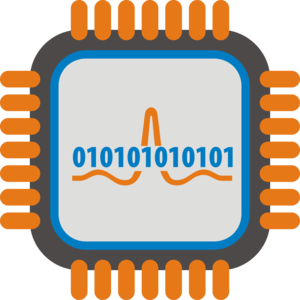
\includegraphics[width=4cm,height=4cm,keepaspectratio]{nucleus}
}
    child[concept color=green!50!white,text=black] { node {Basics\\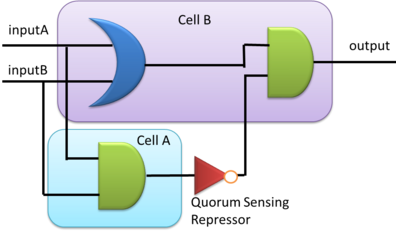
\includegraphics[width=3cm,height=3cm,keepaspectratio]{gates_composed_2}}
        child { node {Boolean Algebra} 
            child { node {Number Systems} 
                child { node {Signed/Unsigned} }
                child { node {1's copmliment} }
                child { node {2's copmliment} }
                child { node {Overflow} }
            }
        }
        child { node {Logic Gates} 
            child { node {OR\\
\includegraphics[width=1.5cm,height=1.5cm,keepaspectratio]{or_gate}} }
            child { node {AND\\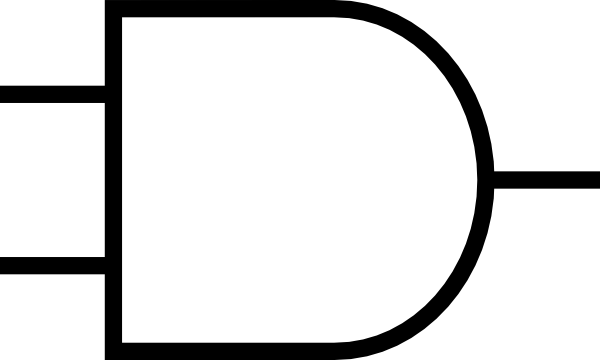
\includegraphics[width=1.5cm,height=1.5cm,keepaspectratio]{and_gate}} }
            child { node {NOT\\
\includegraphics[width=1.5cm,height=1.5cm,keepaspectratio]{not_gate}} }
            child { node {XOR\\
\includegraphics[width=1.5cm,height=1.5cm,keepaspectratio]{xor_gate}} }
        }
        child { node {Minimization\\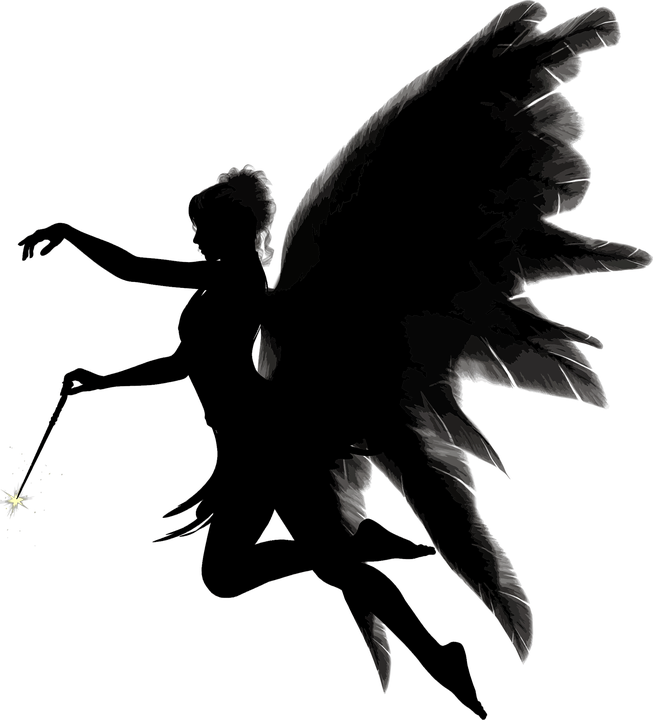
\includegraphics[width=1.5cm,height=1.5cm,keepaspectratio]{fairy_minimize}} 
            child { node {Boolean Algebra} }
            child { node {Karnaugh Maps} 
                child { node {Sum of Products} }
                child { node {Product of Sums} }
                child { node {Don't care} }
            }
        }
    }
    child[concept color=blue!30!white,text=black] { node {Design Approaches\\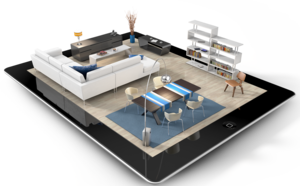
\includegraphics[width=4cm,height=4cm,keepaspectratio]{interior_design}} 
        child { node {Design All Cases} }
        child { node {Speculative} }
        child { node {Pre-Computation} }
        child { node {Design \& Conquer\\
\includegraphics[width=1.5cm,height=1.5cm,keepaspectratio]{sub_trees}} 
            child { node {Break-up} }
            child { node {Stitch-up} }
            child { node {Scenarios} 
                child { node {Comparator} }
                child { node {$2^n$ to 1 MUX} }
                child { node {Multiplier} 
                    child { node {Carry-Save Add} }
                }
                child { node {Ripple-Carry Adder} }
            }
            child { node {Associative Ops} }
            child { node {Non-Associative} }
        }
        child { node {Combine Strategies} }
        child { node {Pipeline} 
            child {node {Registers} }
        }
    }
    child[concept color=orange!50!white,text=black] { node {Combinational Circuits\\
\includegraphics[width=3cm,height=3cm,keepaspectratio]{combo_circuit}} 
        child { node {Multiplexer\\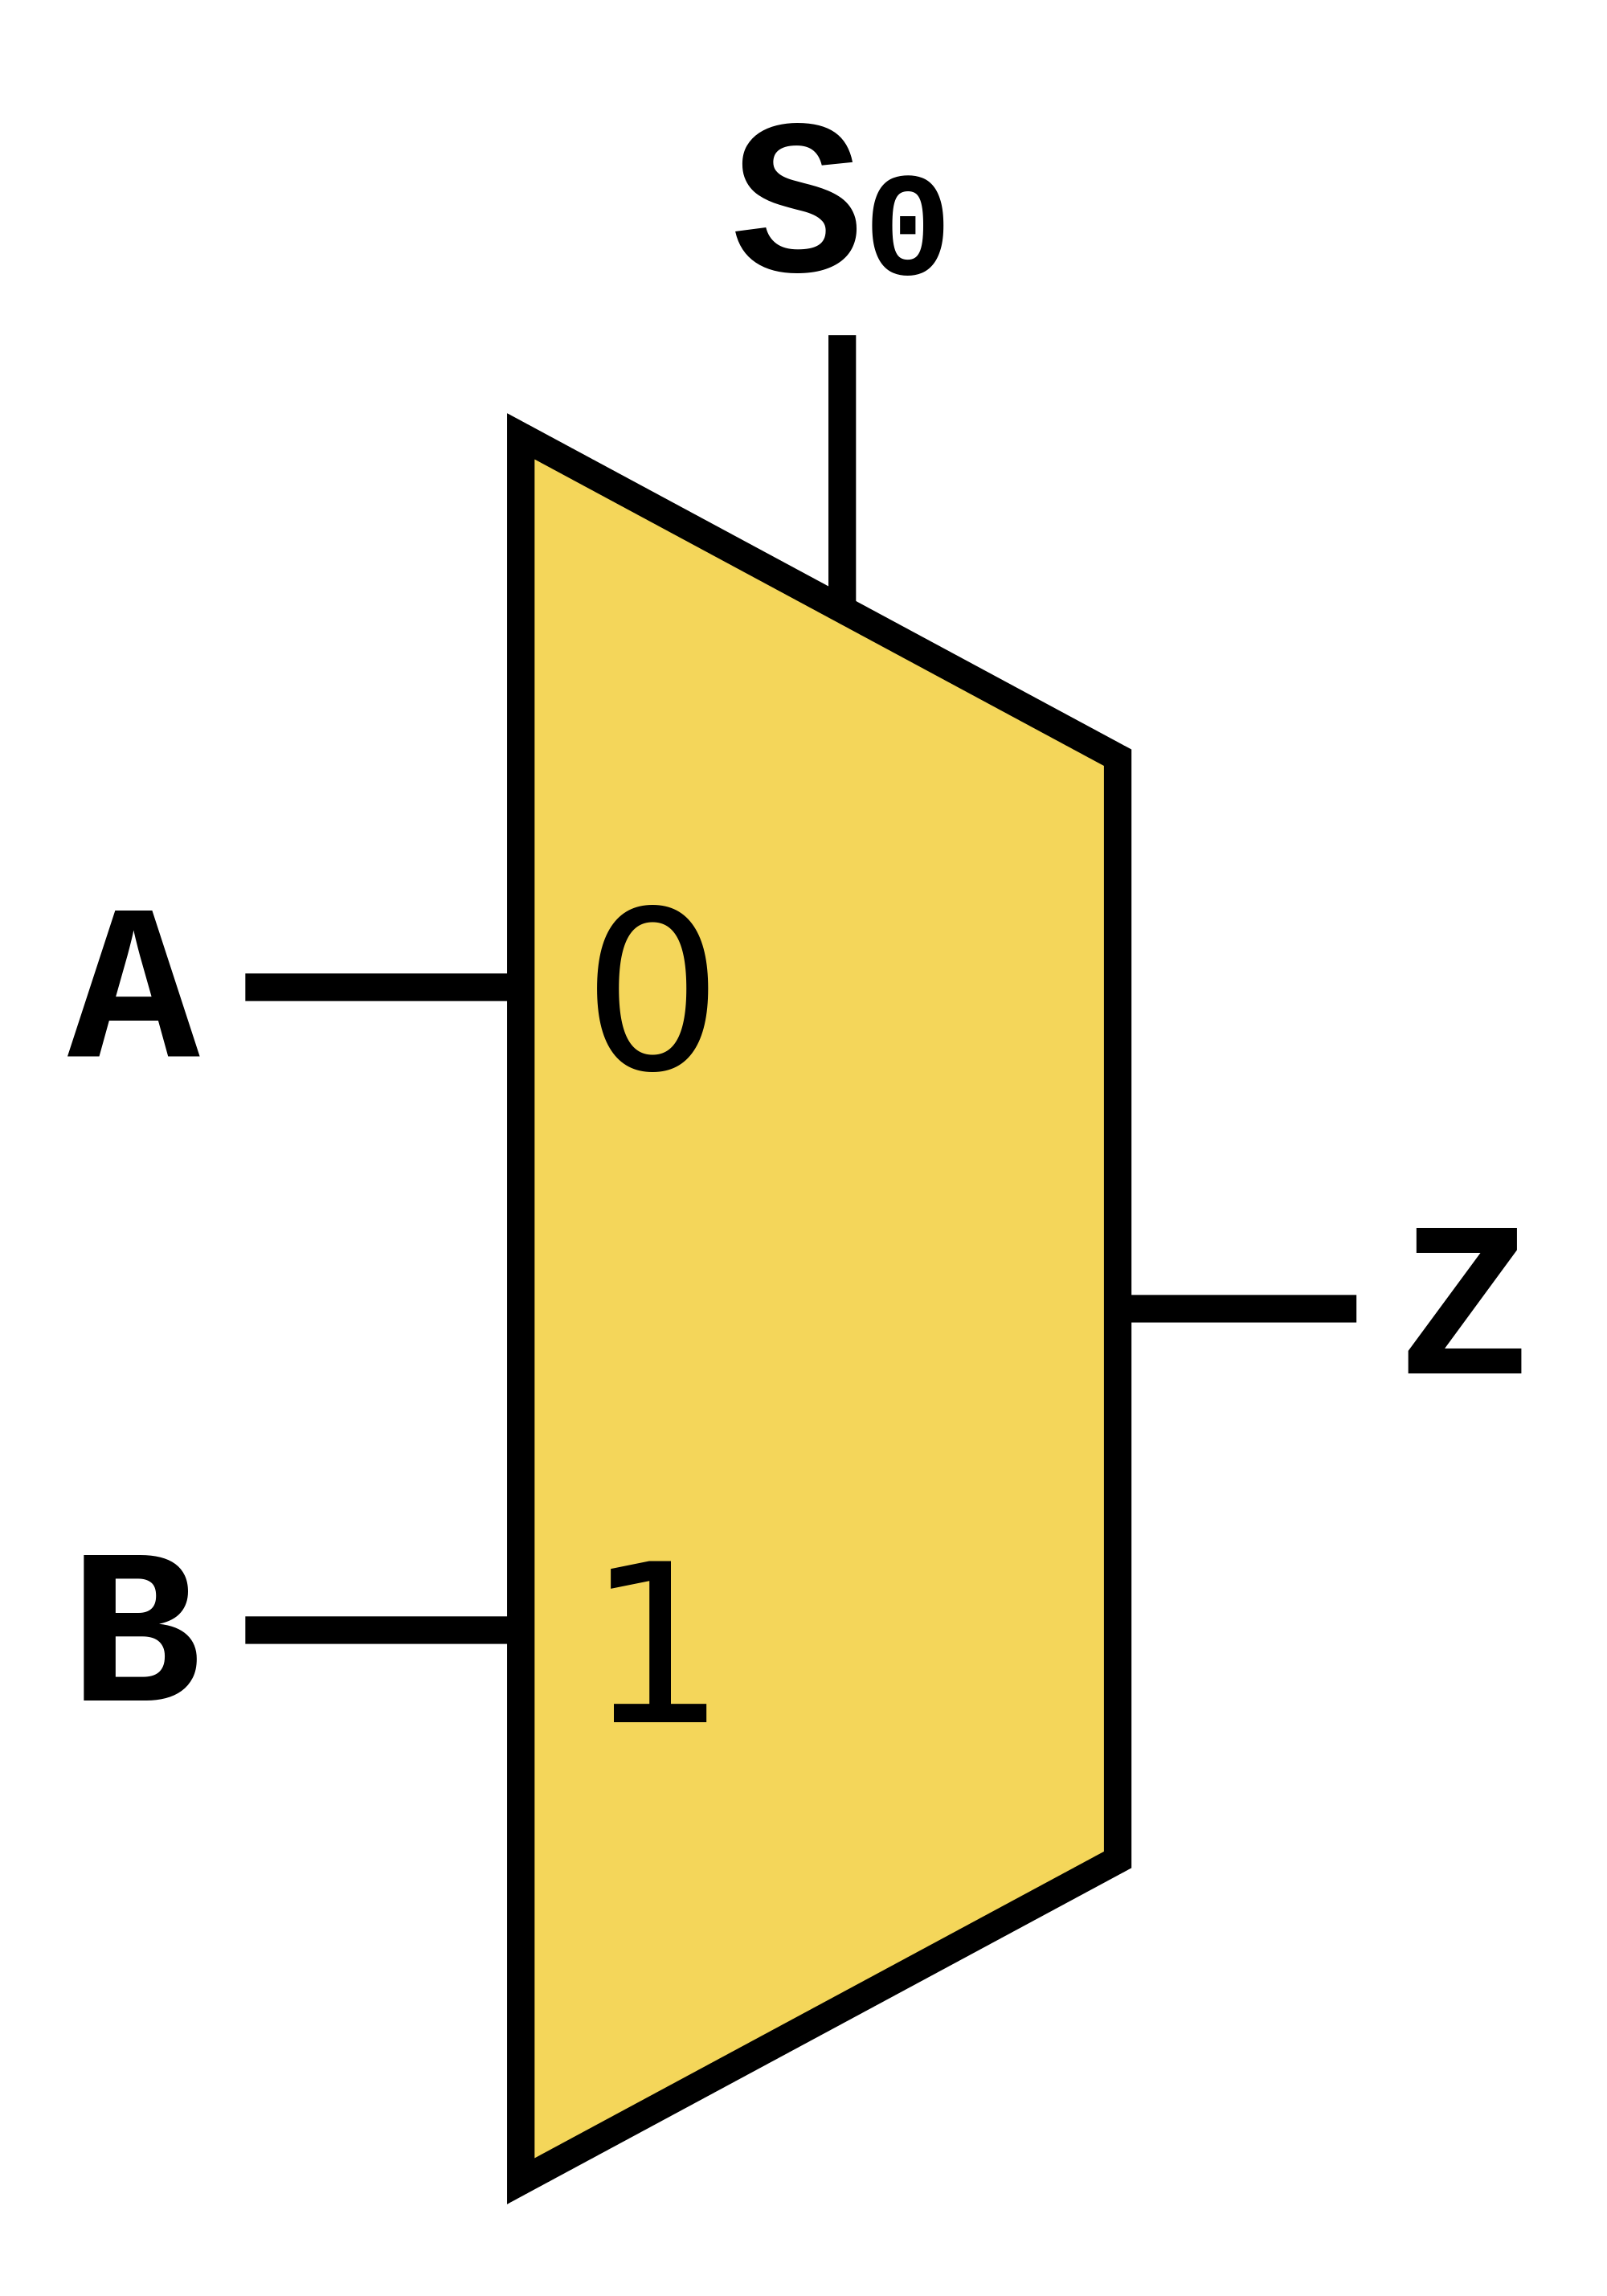
\includegraphics[width=2cm,height=2cm,keepaspectratio]{mux}} }
        child { node {Demux\\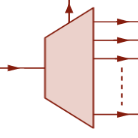
\includegraphics[width=2cm,height=2cm,keepaspectratio]{demux}} }
        child { node {Decoder} }
        child { node {Adder\\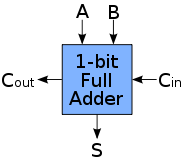
\includegraphics[width=1.5cm,height=1.5cm,keepaspectratio]{full_adder}} 
            child { node {Half} }
            child { node {Full} }
            child { node {Ripple Carry} }
            child { node {Carry Lookahead} }
        }
    }
    child[concept color=purple!30!white,text=black] { node {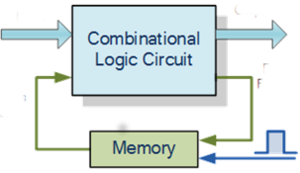
\includegraphics[width=3.5cm,height=3.5cm,keepaspectratio]{seq_circuit}\\Sequential Circuits} 
        child { node {Latches\\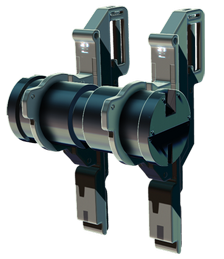
\includegraphics[width=1.5cm,height=1.5cm,keepaspectratio]{latch}} 
            child { node {SR-Latch} }
        }
        child { node {Flip-Flops\\
\includegraphics[width=1.5cm,height=1.5cm,keepaspectratio]{flip_flops}} 
            child { node {Pulse-Triggered} }
            child { node {Edge-Triggered} }
            child { node {J-K} }
            child { node {D-FF} }
        }
        child { node {Registers} 
            child { node {Shift Registers} 
                child { node {Serial Load} }
                child { node {Parallel Load} }
                child { node {Bidirectional} }
            }
            child { node {Serial Adder} }
        }
        child[level distance=5cm] { node {FSMs\\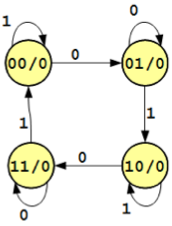
\includegraphics[width=2cm,height=2cm,keepaspectratio]{fsm}} 
            child { node {Moore} }
            child { node {Mealy} }
            child { node {Optimality} }
            child { node {Minimization} 
                child { node {Partitioning} }
                child { node {Implication Table} }
            }
            child { node {Equivalence} 
                child { node {1-equiv} }
                child { node {k-equiv} }
            }
            child { node {Control FSMs} }
            child { node {One-Hot design} }
        }
        child[level distance=5cm] { node {Memory\\
\includegraphics[width=1.5cm,height=1.5cm,keepaspectratio]{ram}} 
            child { node {SRAM} }
            child { node {DRAM} }
            child { node {SDRAM} }
            child { node {ROM} }
        }
        child { node {Programmable Logic} 
            child { node {PLAs} }
            child { node {VLSI\\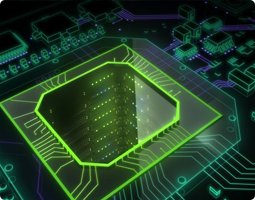
\includegraphics[width=1cm,height=1cm,keepaspectratio]{vlsi}} 
                child { node {CPLDs} }
                child { node {FPGAs} }
            }
            child { node {PALs} }
        }
        child { node {Counters\\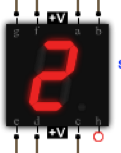
\includegraphics[width=1cm,height=1cm,keepaspectratio]{counter}} 
            child { node {Ripple Binary} }
            child { node {Synchronous Binary} }
            child { node {Synchronous Up/Down} }
            child { node {Parallel Load} }
        }
        child { node {Clocking Methods} 
            child { node {Clock skew\\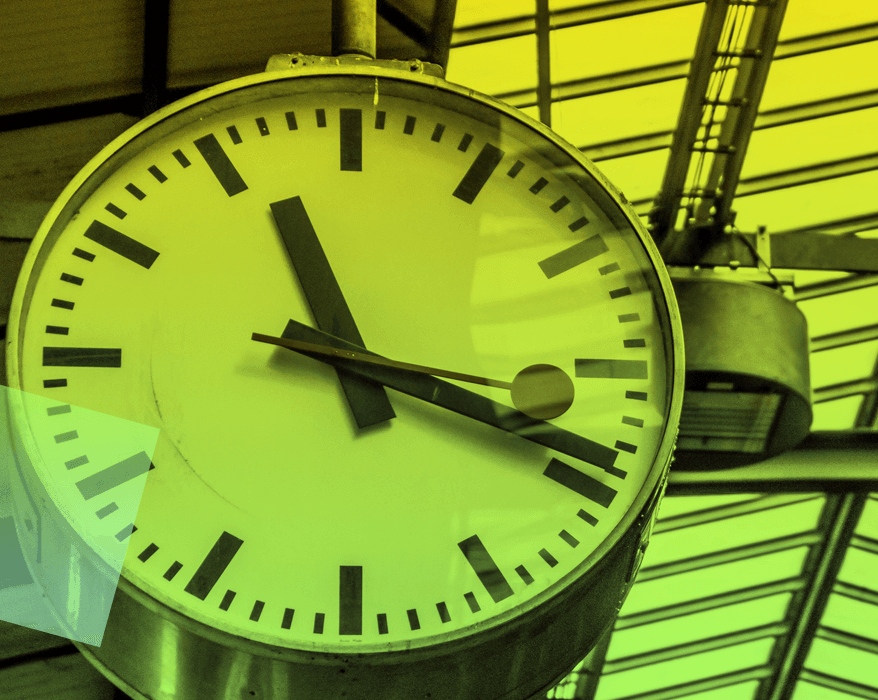
\includegraphics[width=1cm,height=1cm,keepaspectratio]{clock_skew}} }
        }
    }
    child[concept color=red!50!white,text=black] { node {Advanced Minimization\\
\includegraphics[width=3cm,height=3cm,keepaspectratio]{magic_wand}} 
        child { node {QM} }
        child { node {QM+} }
        child { node {QM multi-func} }
        child { node {Petrick's Algorithm} }
    }
    ;
\end{tikzpicture}
\end{document}
